\chapter{Introduction}
A new discipline at the intersection of the development and operation of distributed software systems, known as DevOps~\cite{loukides2012devops}, has seen significant growth recently.  The DevOps community comprises engineers from the development and operations fields, including programmers, testers, quality assurance staff~\cite{rossberg2014collaboration}, system administrators, and others.  These professionals require different tools for carrying out their daily tasks, such as building applications, testing, deploying routines, configuration, automation of utilities, tracking and versioning in systems.  With the advent of cloud computing, a new breed of DevOps professionals,
cloud deployment specialists has emerged. Cloud deployment specialists are responsible for the configuration, provisioning, deployment, testing, and lifecycle management of hosted application solutions. They typically have thorough industry knowledge on all areas 
%security, scaling policies, storage, load balancers, content delivery networks~\cite{buyya2008content} and other areas 
related to the secured hosting and lifecycle management of cloud applications.  

A number of automated tools are available for cloud deployment specialists today.  One such tool is Chef and its associated repository, Chef Supermarket~\cite{Chef_base}. Chef is an application configuration framework that makes it easy to deploy applications on servers on any physical, virtual, or cloud location. The representation of the application resembles code using Chef cookbooks. Another such tool is IBM Bluemix~\cite{Bluemix-dev}, a development and support platform for communities of DevOps users wishing to compose distributed applications out of components drawn from libraries and deploy them at IBM-provided and supported cloud infrastructure.  Both tools however provide only minimal community interaction facilities and do not collect nor leverage any past (historical) experience on application deployments.

Today DevOps cloud deployment specialists exhibit the need to communicate through traditional social networks and other online fora, to exchange views and potential solutions on the cloud deployment of applications.  The current status in this space, however, can be improved.  A motivation for this thesis was the need to improve the efficiency of the interaction and communication between cloud deployment specialists, coupling human interaction with knowledge present in crowdsourced repositories of information, as that would provide them with expert advice and input that is not currently available through the use of automated tooling.
%Having a repository, where they can find the configurations and the executions data of an application and point to those data is valuable since it can make their conversation specific and help them come to more concrete conclusions.

The topic of this thesis is thus the design and implementation of a social networking architecture targeted for cloud deployment specialists engineers.
This social network architecture binds several social networking concepts such as personal messaging, groups, live feeds, etc. with software-engineering concepts such as the composition, deployment, monitoring, and analysis of executions of applications.  The architecture integrates social networking with knowledge present in a repository of cloud applications and infrastructure description based on Cloud Application Modelling and Execution Language (CAMEL)~\cite{paasagedeliverable212}. 
%This CAMEL repository brings to several benefits to the DevOps community.
Among the range of possible DevOps tasks, the design of the social network architecture puts special focus on one of the most challenging tasks of cloud deployment specialists: selecting the most appropriate deployment configuration for an application. This is especially challenging in a multi-cloud setting due to the large diversity of deployment possibilities and tradeoffs. 

Currently DevOps users work with a small set of well-understood deployment options, missing on opportunities for improving performance, reliability and/or lower cost. Investigation of new options involves time consuming testing over new infrastructures. Discussing those topics with the community in online social or technical forums may provide insight over deployment options; however, the answer to a hard question often needs to be backed by experimental data that is not readily available. 

An integrated environment such as proposed in this thesis, comes to solve the above issues by enriching user interactions with structured references to applications and their components, execution data, and mined knowledge from real deployments. Mined knowledge can be combined with user activity and profiles to provide personalized suggestions and hints.  An improved mode of user interaction is expected to result in stronger incentives for DevOps users to contribute information to the underlying repositories. Richer content should lead to better quality of mined knowledge, benefiting the DevOps community and providing further incentive for contributions.  The social networking platform is designed to be closely integrated with a set of information repositories satisfying the following requirements: 
(R1) handle entire applications rather than just software components; (R2) abstract application structure through software modeling; (R3) capture and analyze application runtime performance.  Existing repositories used in this thesis include Chef Supermarket and the PaaSage CAMEL repository.

Broadening the focus from individual software components to entire applications and analyzing their execution data, can provide answers to many interesting questions and support community discussions and arguments with hard data. 
We believe that these requirements can provide software developers with strong urge to contribute, leading to the sustainability and growth of information and derived knowledge in the repository.

This thesis is structured as follows: Section~\ref{sec:background} provides background on application models and the CAMEL repository developed in the context of PaaSage EU project. Chapter~\ref{sec:related} describes previous work on the scalability of social networking platforms through caching mechanisms and on topic classification. In Chapter~\ref{chap:implementation}, we describe the implementation of the social networking architecture\footnote{The user interface (UI) design and usability evaluation was the result of a collaboration with the Human-Computer Interaction (HCI) laboratory of ICS-FORTH~\cite{magoutis2015design}.}, and in Chapter~\ref{chapt:evaluation} we present our evaluation. Finally, in Chapter~\ref{sec:conclusions} we present our conclusions.

\section{Background}
\label{sec:background}
This section presents an overview of the descriptions of the application models that are available on the Social Network Platform and a summary of the technologies that are used by the PaaSage in order to assist the cloud deployment specialists to deploy the aforementioned application models.

Application models inside social network platform are described in CAMEL. CAMEL integrates various domain-specific languages (DSLs).
DSLs provide a notation tailored towards an application domain and are based on the relevant concepts and features of that domain. As such, a DSL is a means to describe and generate members of a family of programs in the domain. 
These DSLs cover a wealth of aspects of specification and execution of multi-cloud applications like CloudML, Scalability rules, WS Agreement, Saloon and Historical Execution Data. 

CloudML~\cite{FerryRossiniCMS13} is a recent approach that focuses on the provisioning and deployment of multi-cloud applications, is built upon MDE techniques and methods, and provides a models@run-time~\cite{models-runtime} environment for enacting the provisioning.  WS Agreement~\cite{andrieux2007web} is a Web Services protocol for establishing agreement between two parties, such as between a service provider and customer. Saloon ~\cite{quinton2013towards} is an approach that uses models to represent clouds variability, as well as ontologies to describe the heterogeneous aspect of the cloud ecosystem. The CAMEL model assembles all those DSLs as shown in Figure~\ref{fig:dsls}.

CAMEL is using the Eclipse Modelling Framework (EMF)~\cite{steinberg2008emf} on top of the Connected Data Objects (CDO)~\cite{cdomodel}~\cite{paasage-d4.1.1}. Application Models are persisted on the CDO repository. EMF is used as a building tool for the application models. CAMEL model specification is written in XMI format (XML Metadata Interchange) which is a standard for exchanging metadata information via Extensible Markup Language (XML). Thus, XMI consists the main describing system of CAMEL and EMF provides tools that enable viewing and command-based or tree-based editing of the application models. 

\begin{figure}[h]
	\centering
	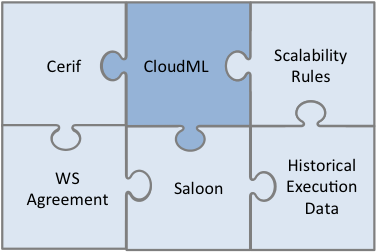
\includegraphics[width=0.6\textwidth,natwidth=200,natheight=150]{./fig/dsl.png}
	\caption{CAMEL DSLs}
	\label{fig:dsls}
\end{figure}

A representation of a model using the EMF editor is shown in Figure~\ref{fig:app_view_emf}. The Cloud Deployment Specialist can add all the information needed for the deployment of the application. For example, the figure~\ref{fig:app_view_emf} shows the ``Deployment Model'', which contain the configuration of CloudML. This information is needed for the application to be deployed. The ``Provider Model'' and the ``Location Model'' contains information about the Cloud Providers that will be used for this specific deployment of the application. This application has not any historical executions yet, but after the deployment it will be populated with those data.
 
The CAMEL repository is currently being populated with a wealth of information from multi-cloud deployments of various distributed applications~\cite{Papaioannou2013}. Also, SNP performs analytics over the CAMEL repository to extract knowledge about deployments characteristics that work best for certain applications and use it in the context of the professional network.

\begin{figure}[h]
	\centering
	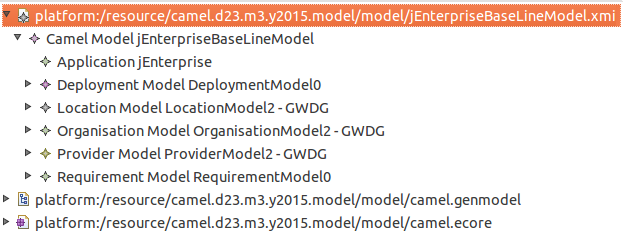
\includegraphics[width=0.8\textwidth,natwidth=200,natheight=150]{./fig/camel_model_example.png}
	\caption{An application model view from EMF editor}
	\label{fig:app_view_emf}
\end{figure}

The Social Network Platform proposed in this thesis is part of the PaaSage EU Project~\cite{paasage}.
The PaaSage perspective is to be a tool for a cloud deployment Specialist to leverage the complex task of deploying an application to the clouds. Usually, a cloud deployment specialist could easily learn the interface and features of one Cloud provider, but it would be very costly and time consuming to leverage the development to many providers. It is a real challenge to orchestrate the simultaneous deployment to many different Clouds at the same time. The main objective of PaaSage is to assist the developer to deal with difficult deployment scenarios through automatic cloud deployment. In order to satisfy this, several components are included to the PaaSage ecosystem. The Profiler components read the CAMEL models and convert them into a constraint programming model by defining the variables of the model, their domains, and the constraints that must be satisfied by the deployment. Also, the Profiler checks all constraints of the CAMEL model and sets the domains of the variables accordingly. The reasoning component analyses the model and finds how deployment candidates should be evaluated. Once a solution has been found, the reasoning component converts the model to Cloud Provider Specific Models (CPSM) for the providers involved in the proposed deployment. The adapter component takes the CPSMs, produces and validates a configuration plan, and sends this plan to the execution ware. The execution ware~\cite{baur2014towards} receives the deployment plan from the adapter and enacts the deployment of the application on the selected providers. Furthermore, the execution ware interacts with the Cloud providers, acquires the virtual machines, configures them and launches the user application on the set of those machines. Once the machines are running, the execution ware collects sensor data for the running application, triggering re-configurations if necessary.

The Social Network Platform brings to the DevOps users a friendly interface to browse, discover, view and discuss Application Models. Furthermore, it presents a way to deploy and run these Application Models, by using the previously mentioned components under the hood, and mines their execution history data.

The key contributions of this Social Network Platform (SNP) are the following:
\begin{itemize}
\item The SNP binds all the Social Networking aspects such as friends, new feeds, personal messages etc. with the engineering aspects of creating and deploying application models.
\item The SNP brings the execution histories of the CAMEL applications in the light, providing the end users the ability to browse, discuss, point and find essential information needed for other applications.
\item The SNP uses the best known practices both for the front end viewing system and the back end technology.
\item The SNP runs on a horizontal scale architecture with memcached at the back end to reach near real time interaction. 
\end{itemize}


